% vim: set filetype=tex:ai:et:sw=4:ts=4:sts=4:tw=80
%----------------------------------------------------------------------------------------
%	PACKAGES AND OTHER DOCUMENT CONFIGURATIONS
%----------------------------------------------------------------------------------------

\documentclass{article}

\usepackage[utf8]{inputenc}
\usepackage{fancyhdr} % Required for custom headers
\usepackage{extramarks} % Required for headers and footers
\usepackage{graphicx} % Required to insert images
\graphicspath{ {./pic/} }
\usepackage[backend=bibtex,style=numeric,sorting=none]{biblatex}
\usepackage{url}
\usepackage{mathtools}
\usepackage{hyperref}

% Margins
\topmargin=-0.45in
\evensidemargin=0in
\oddsidemargin=0in
\textwidth=6.5in
\textheight=9.0in
\headsep=0.25in

\linespread{1.1} % Line spacing

%----------------------------------------------------------------------------------------
%	TITLE
%----------------------------------------------------------------------------------------

\title{
\textmd{IA158 Real Time Systems}\\
\textmd{\textbf{Legway}}
}

\author{\textbf{Jan Dupal, Adrian Farmadin, Peter Kotvan, Vít Šesták}}
\date{11. 5. 2014} % Insert date here if you want it to appear below your name

\bibliography{./bib/bibliography.bib}

%----------------------------------------------------------------------------------------

\begin{document}

\maketitle

\section{Introduction}

Our project is inspired by Segway, two-wheeled, self-balancing, battery-powered
vehicle. \cite{segway} \cite{wseg} As the Lego robotic set did not contain
gyroscopes we used light sensor for measuring the tilt of the robot as can be
seen on figure~\ref{fig:legway}. The sensor is located under the Lego brick.

\begin{figure}[h]
    \centering
    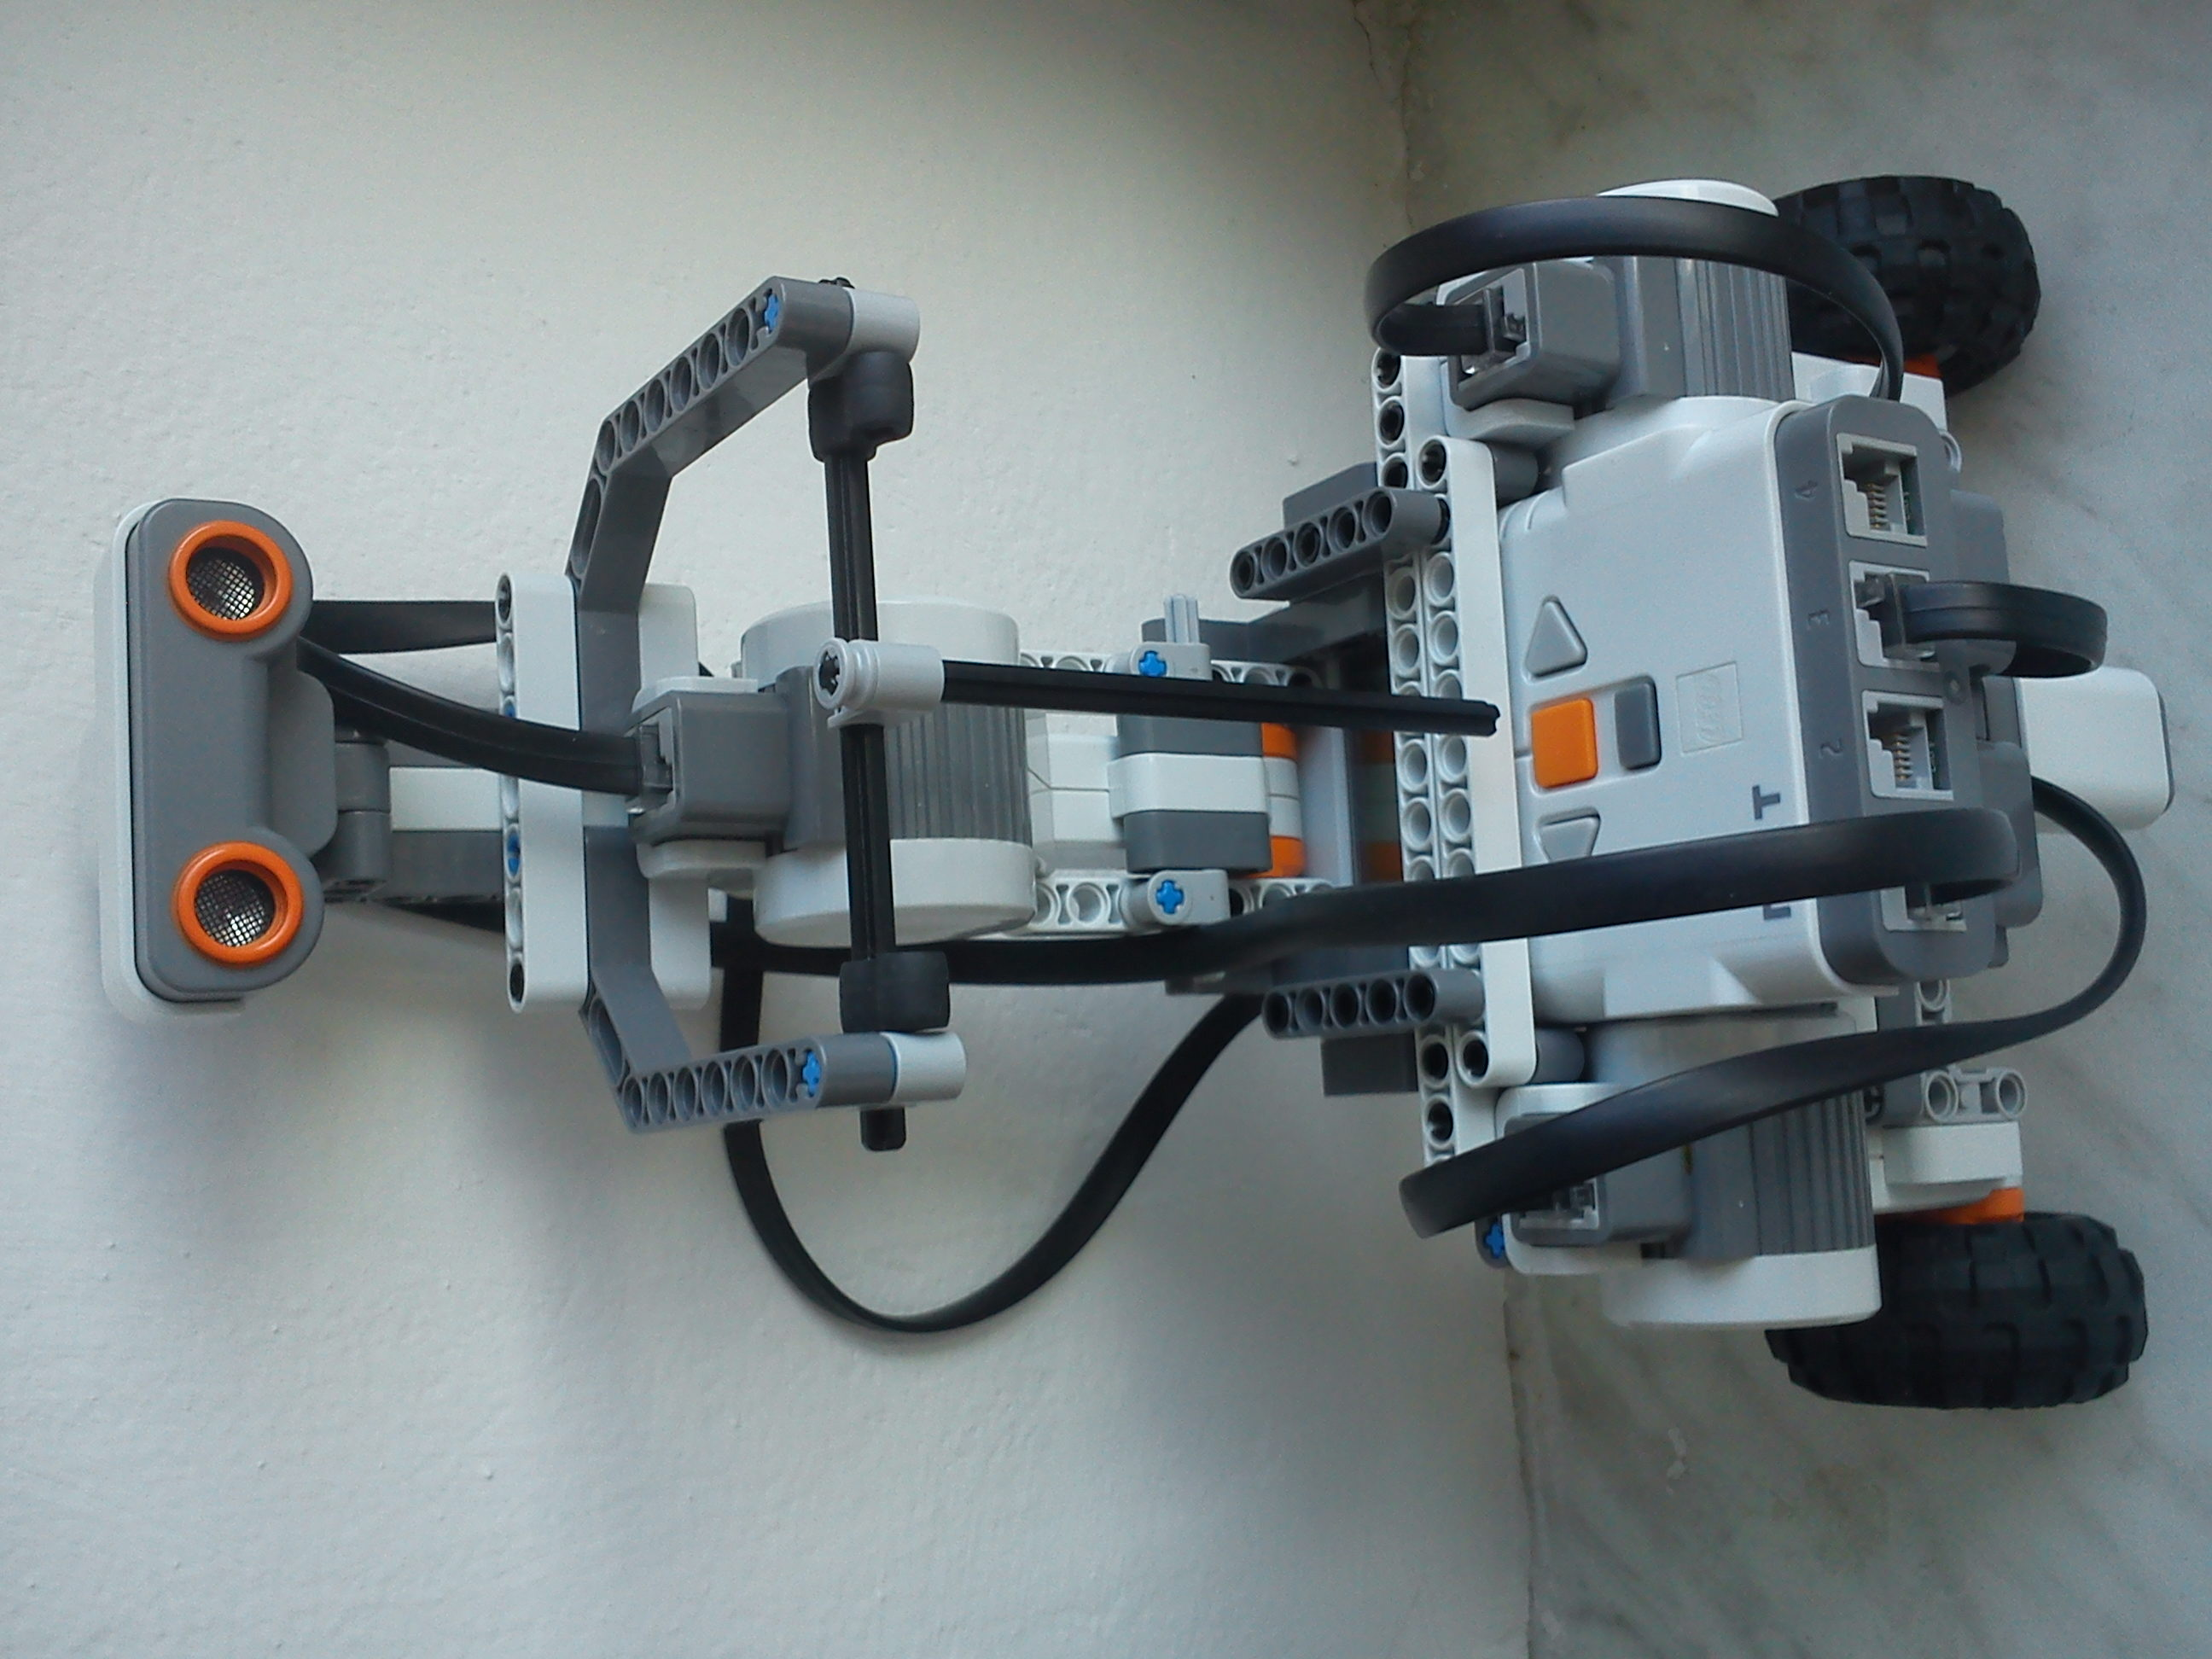
\includegraphics[width=7cm, angle=270]{legway}
    \caption{Legway}
    \label{fig:legway}
\end{figure}

The communication with Lego brick is done over bluetooth. Initially we intended
to use ultrasonic sensor to avoid obstacles but later we decided to remove
unnecessary parts to lower the centre of gravity to solve our problems with
balancing.

For different parts of the project our team used different programming
languages. The main program of the robot is written in NXC \cite{nxc} which is a
language very similar to C. Testing module for bluetooth communication is
written in Ruby and finally the application for controlling the segway is
written in Scala.

Unfortunately during our work on this project we experienced display failure on
Lego brick two times. This caused delay in our work and the second malfunction
prevented us from merging the codebases of team members and from enough
experimentation with controller parameters as our team used the display for
debugging purposes.

\section{Controller}

Control theory is a branch of science that studies the behavior of dynamical
systems and describes the ways of controlling them. To enable our robot to
balance itself we had to implement basic PID controller with with feedback loop.
Figure~\ref{fig:loop} shows basic closed-loop controll system.

\begin{figure}[h]
    \centering
    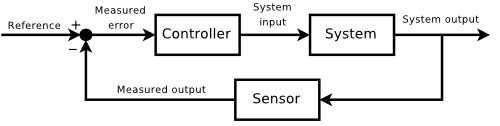
\includegraphics[width=9cm]{loop}
    \caption{Feedback loop \cite{wloop}}
    \label{fig:loop}
\end{figure}

\subsection{Discrete PID}

We have chosen discrete version of PID controller because of it's simplicity and
easiness of implementation however this type of controller is meant to be used
with identified linear systems and we know that our system is not linear and we
have no means to identify it. We assumed that the robot will behave linearly
close to point of equilibrium since the equations describing the system can
linearized using Taylor series and terms with power of two and higher could be
neglected.

Standard form of PID controller look is

\begin{equation} \label{eq:pid}
    u(t) = K \left( e(t) + \frac{1}{T_i} \int_0^t e(\tau)d\tau + T_d
        \frac{de(t)}{dt} \right)
\end{equation}

\noindent where $e(t)$ is the error, the difference between required value and
the output of the system and $u(t)$ is the controller output. Performing Laplace
transformation \cite{lt} on (\ref{eq:pid}) we get

\begin{equation}
    G(s) = K \left( 1 + \frac{1}{sT_i} + sT_d \right)
\end{equation}

\noindent or the parallel form

\begin{equation} \label{eq:para}
    u(t) =  K_pe(t) + K_i \int_0^t e(\tau)d\tau + K_d
        \frac{de(t)}{dt}\end{equation}

\noindent with its Laplace transform

\begin{equation}
    G(s) = K_p + \frac{K_i}{s} + sK_d
\end{equation}

\noindent where we can simple convert the constants $K_p = K$, $K_i =
\frac{K}{T_i}$ and $K_d = KT_d$. These constants, sometimes denoted $P$, $I$, $D$ are the proportional gain,
integral time and the derivative time respectively.

\begin{figure}[h]
    \centering
    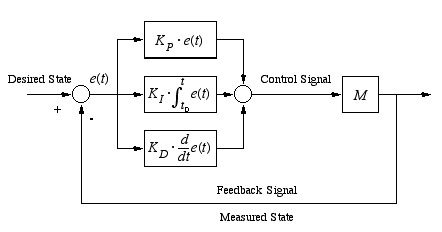
\includegraphics[width=8cm]{pid}
    \caption{PID controller in controll loop \cite{pidpic}}
    \label{fig:pidpic}
\end{figure}

Since we need to use the controller in digital form we need to use discrete form
of PID controller sometimes called PSD controller with S denoting sum instead of
integral. This can be achieved with Z-transform of the equation (\ref{eq:para}).
\cite{zt}

\begin{equation}
    U(z) = \left( K_p + \frac{K_i}{1-z^{-1}} + K_d\left(1-z^{-1}\right) \right)E(z)
\end{equation}

\begin{equation} \label{eq:zpid}
    U(z) = \left( \frac{\left( K_p + K_i + K_d\right) + \left(
    -K_p-2K_d\right)z_{-1} + K_dz^{-2}}{1-z^{-1}} \right)E(z)
\end{equation}

\noindent We have defined

\begin{eqnarray*}
    K_1 &=& K_p + K_i + K_d \\
    K_2 &=& -K_p-2K_d \\
    K_3 &=& K_d
\end{eqnarray*}

\noindent to be able to derive difference equation from (\ref{eq:zpid}).

\begin{equation}
    u[k] = u[k-1] + K_1e[k]+K_2e[k-1]+K_3e[k-2]
\end{equation}

In our final implementation of PSD controller we used slightly different
equations that incorporate also the sampling rate parameter $T_s$. \cite{tar}

There are several methods that could be used to determine the constants of PID
controller for example Ziegler-Nichols method or Cohen-Coon method. However
these methods need more information about controlled system than we had and they
need ways to measure various parameters of the system. Hence we tried to set
parameters experimentally assuming that in the state of equilibrium there is
zero error, so we decided to set integral time to zero and change only
proportional and derivative gain.

\section{Bluetooth}

In order to provide some kind of interactivity we've decided to include remote control. Bluetooth interface was obvious choice as wired connection would affect stability of the vehicle.

\subsection{Requirements}
Our remote control is very simple. It just controls the requested speed of the Legway device. The actual speed may be, however, different, which may be caused by various physical limits. For example, we can't switch from stopped Legway to full speed instantly.

\subsection{Bluetooth with NXC}

Although the brick is Bluetooth-enabled, NXC does not provide capability to use RFCOMM profile (i.e. serial port emulation) directly. There is implemented a higher level protocol on top of RFCOMM. The protocol distinguishes between "master" (i.e. the device that initiated the connection) and "slave" (i.e. the other device).

The protocol allows us to send various commands such as run programs, play tones etc. The most important part of the protocol are command queues. There are several message inboxes with a limited capacity. All inboxes are stored on the "slave" device. The "master" device can push a new message and poll for new messages. The "slave" device does not send the "master" any message until "master" asks the "slave" to do so. \cite{nxt-bt}

When "master" is waiting for a message from "slave", it must poll. It can be a serious performance issue in poorly designed protocols on top of that, especially with the poor Bluetooth radio device that has a significant delay (around 100 ms) when switching between receive and send mode.

It was a surprise that NXC seems to support secured Bluetooth connections.


\subsection{Legway specific challenges}

\subsubsection{Lost connection and delayed messages}

There may be various issues with Bluetooth connections and remote control. In addition, even if we have a secured connection, an adversary still may delay some packets, which could be generally harmful in realtime environments, since executing a delayed command may do something undesired. The goal was to protect the Legway from delayed commands and lost commands. When there is such connection related issue, Legway does not know what the remote user intends to do. However, it can at least try to behave safely when such issue occurs. We assume that the safest behavior in such case is stopping the Legway. It can of course depend on the environment in the real world.

Fortunately, lost connection (even before timeout) and delayed commands can be detected by similar mechanism:

\begin{enumerate}
\item The remote control should poll and periodically confirm that the connection is alive. If there is no activity seen from the remote control (e.g connection has been lost, the remote control has run out of battery energy or the remote control has a kernel panic), the Legway should stop.
\item All the messages from remote control should contain some time information that allows us to know that the message is too old to be processed.
\end{enumerate}

We have decided not to make special keep-alive messages in order to simplify the design. When a connection is initiated, there is only one type of messages. These messages contain two values. The first one is the requested speed (from -5 to 5). The second one is the `validUntil` value, which is a time. (We will discuss the \textit{time} later.) If the message is being processed after `validUntil`, it is simply ignored. If there is no new message until `validUntil` time instant, the requested speed is automatically set to zero in order to prevent crashes etc., assuming a trouble with the connection.

\subsubsection{Syncing the time}
We don't assume that both parties have configured the time correctly. We will however assume that both clocks have the some speeds. We assume that Legway is too slow to experience noticeable time dilation known from the theory of relativity. 

So, we can measure time from the beginning of the communication. This is not so simple, however. There are several ways to do that:

\begin{enumerate}
\item Assume that delays are negligible and start the time measurement on the initiator side after the `hello` message is sent. This is how it is implemented currently. It however allows an adversary in the middle to delay the initial message and then make variable delay to other messages.
\item Wait for the system confirmation packet of the `hello` message and then start the time measurement. (Assuming that we will require confirming the `hello` message.) This however does not guarantee us that the application has processed the hello message. It does not even guarantee us that the application is running.
\item After the `hello` message is sent, we will poll for a reply message. The the reply message is received, the time measurement begins. The polling will definitely increase the connection time, but unlike the other ways, this way is reliable. It guarantees that $legwayTime \geq remoteControlTime$, which is required for `validUntil` to work correctly in the defensive way. This is how we wished to implement it. We haven't this done, because the brick stopped working.
\end{enumerate}

\section{Scheduling}

Naturally both PID Controller and Bluetooth remote control are timing-critical components. Failure in them may cause:

\begin{enumerate}
\item Delay between two samples from the light sensor may cause a delay in reaction of motors, thus failing to keep the vehicle in equilibrium.
\item Long period of mailbox fetching causes queue overflow, thus loss of commands.
\item Also timing is crucial for handling of lost connection -- shorter period means quicker fall-back reaction (i.e. halting the vehicle).
\end{enumerate}

We have planned to setup scheduling with fixed periods and phase shifts of individual tasks. Initially both components were developed (incl. scheduling) separately and later they were merged together. However the malfunction prevented us from measuring execution time of individual tasks, thus we were unable to prepare correct schedule for tasks.



\subsection{PID}

Experiments have shown that PID Controller task has to be run with period 5 to 10 ms (100 to 200 Hz) in order to drive the motors properly. Although the CPU would be able perform the task with even higher frequency, the period is fundamentally limited by the free play of the employed motors and gearboxes.

\subsection{Bluetooth}

Two tasks for responsible for remote control has to be scheduled:

\begin{description}
\item[Message receiving task] periodically fetching the head of mailbox queue. As the NXT communication protocol sends ACK to each message received from 'master' device (thus switching radio from \textit{rx} to \textit{tx} mode and back) it is unnecessary to execute this task with period shorter than 100 ms.
\item[Command validity task] ensures that issued commands have only time-limited influence on the system in case of e.g. lost connection. In these cases this task sets requested velocity to zero.

To prevent race-conditions this task is also responsible for setting the requested velocity according to received commands. Therefore this task should have period similar to the previous task, ideally with slight phase shift to ensure the shortest time between receiving a message and setting velocity parameter of PID.
\end{description}

The planned period was 100 ms (10 Hz) for both tasks with 50 ms phase shift. Thus tasks would be altering with period 50 ms.

\subsection{Debug tooling}

Various kinds of debug output drawn on the integrated LCD screen proved to be very helpful part of the development process. The period of these task can be set to quite high values (tenths to ones of second, 1 to 10 Hz) to affect the system least as possible.

\section{Conclusion}

As was already mentioned in introduction our work was slowed down by two
failures of Lego Mindstorms brick. That is why our project is not completely
finished. During testing of the controller we experienced that the sensor is
sensitive to change of light conditions. The controlling mechanism alone worked
but we suspect that the motors could not deliver enough power soon enough to
balance the robot before it falls down. This problem could be probably fixed
with better setting of PSD controller constants.

\printbibliography

\end{document}

